\chapter{\emph{AlgorAI}: creación de una pieza de arte sonoro generada con ayuda de GPT-4}
\label{chap:algorai}

% \defaultFontEpigraph{Imagination Is All You Need!\dots}{\cite{erkerImaginationAllYou2023}}
\defaultFontEpigraph{Imagination Is All You Need!}{Erker, Schaffer, y Spanakis (2023)}

% \captionqranexo{}{https://vimeo.com/906122849?share=copy}{video}
% \vspace{1cm}

Una de las actividades planificadas en el marco de esta investigación ha sido la creación de una pieza de arte sonoro usando de la interacción con \gls{llm}. La pieza resultante, titulada \emph{AlgorAI}, puede ser escuchada en el enlace del código QR de la Figura \ref{fig:sonograma_algorai}. En este capítulo se describirá el proceso de creación de la pieza, los materiales sonoros generados por GPT-4 que han sido utilizados en la misma, y los resultados de la interacción humano-\gls{llm} en el proceso de composición.

\begin{figure}[H]
    \captionqr{Sonograma de una parte de la pieza electroacústica \emph{AlgorAI}}{Sonograma de una parte de la pieza electroacústica \emph{AlgorAI}.}{https://vimeo.com/906122849?share=copy}{video}
    \centering
    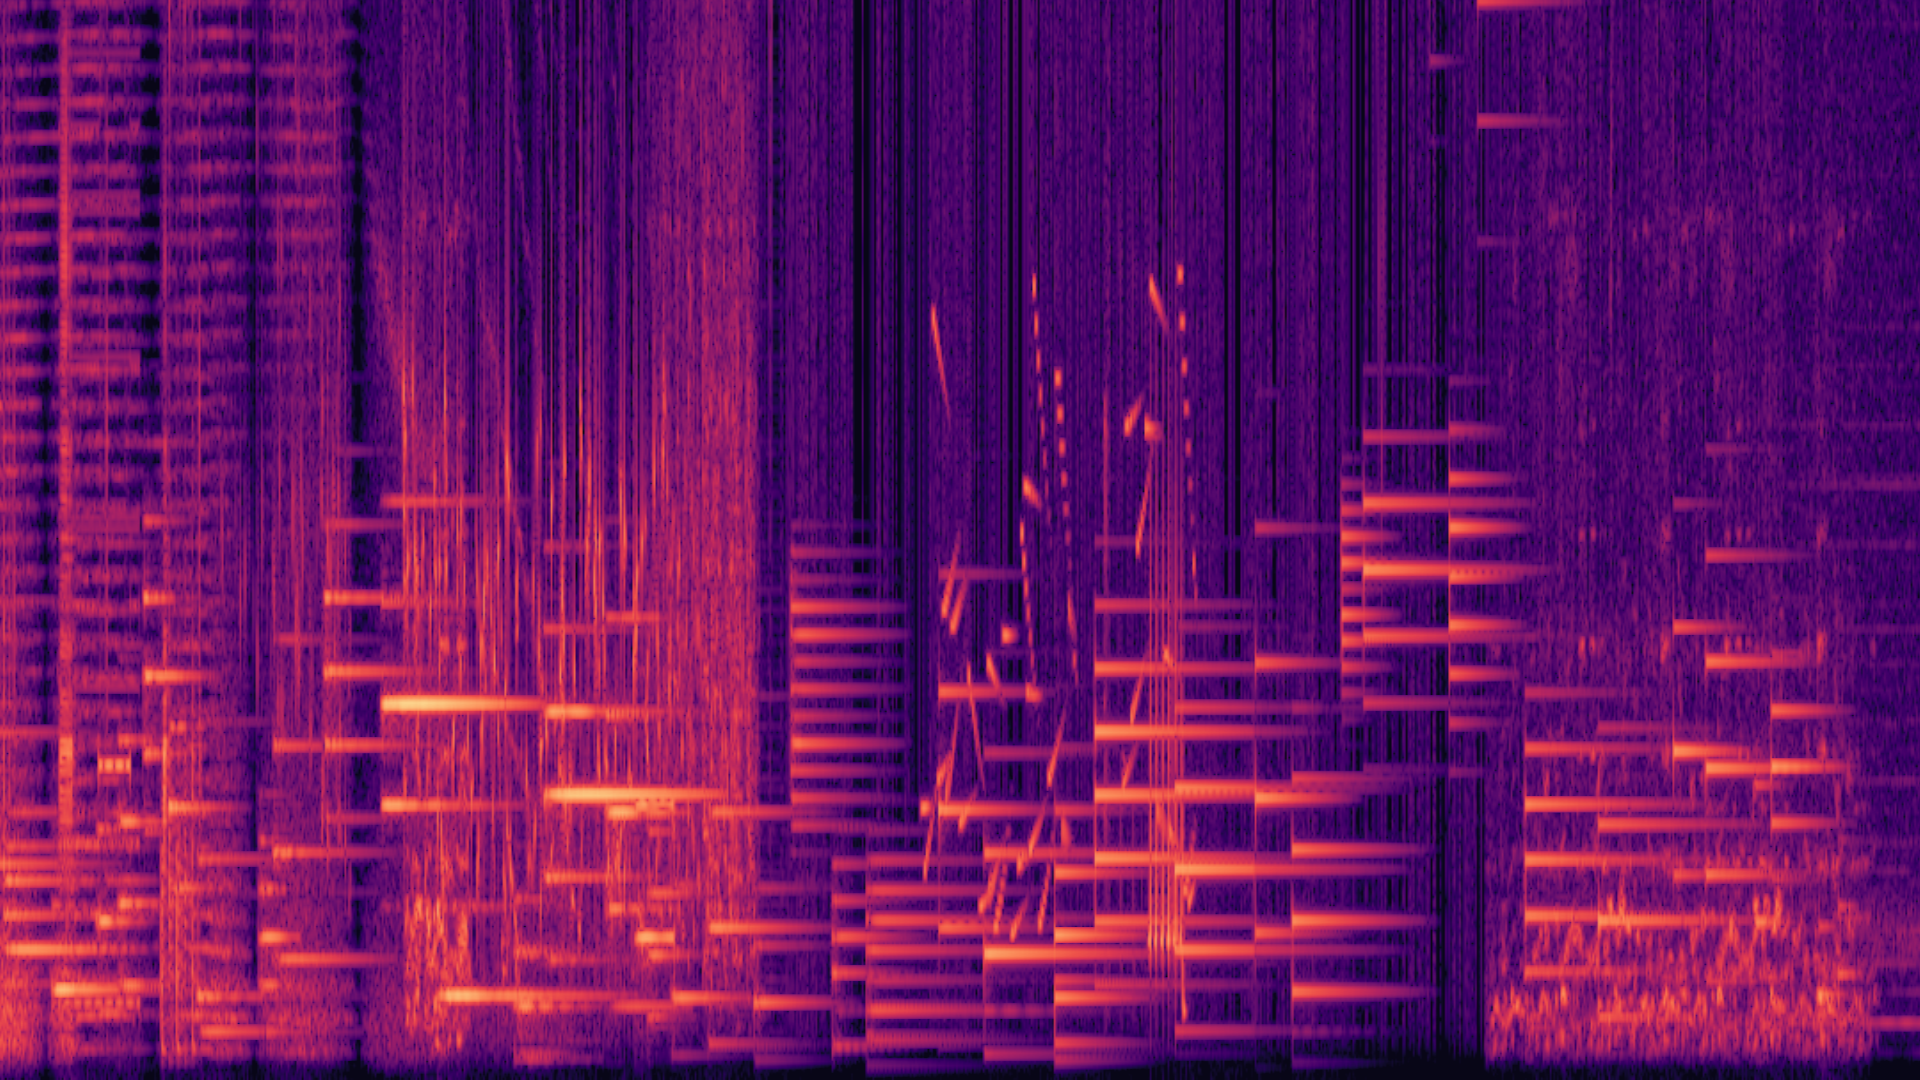
\includegraphics[width=0.8\textwidth]{./figuras/sonograma_02.png}
    \note{Se puede apreciar parte de la trama polifónica creada por los diversos materiales sonoros que la componen. El código QR enlaza con un vídeo que ofrece la escucha de la pieza.}
    \source{\propio}
    \label{fig:sonograma_algorai}
\end{figure}

Como consecuencia de las pruebas y prácticas llevadas a cabo con la \gls{api} y el Playground de OpenAI para este trabajo, se generaron decenas de archivos con código cuyo resultado sonoro fue juzgado de cierto interés. Estos bloques de código están escritos tanto en SuperCollider como en Tidal Cycles. En el primer caso responden a peticiones muy concretas de texturas, timbres o sucesiones sonoras, en el Playground o en ChatGPT; en el segundo, a sesiones de \emph{live coding} compartidas, asistidas por la \gls{api} en \emph{AlgorAI}.

Ninguna de las construcciones de código conseguidas responden a un plan de una pieza completa, sino, más bien, a texturas sonoras continuas o con pocas variaciones en el tiempo. Por esta razón, el planteamiento de composición de una pieza a partir de estos materiales ha sido organizado absolutamente por el compositor-investigador. Se ha optado por organizar los sonidos elegidos en la \gls{daw} \emph{Ardour}. Los procesados y efectos aplicados han sido mínimos, con el fin de mantener la esencia de los sonidos generados por GPT-4, limitándose a filtrados, cortes y compensación dinámica entre elementos. 

% La Figura \ref{fig:ardour} muestra la organización de los sonidos en la DAW.

% \begin{figure}
%     \captionqr{Captura de pantalla de la DAW Ardour con los sonidos generados por GPT-4 organizados por pistas en una composición de arte sonoro.}{https://vimeo.com/906122849?share=copy}{video}
%     \centering
%     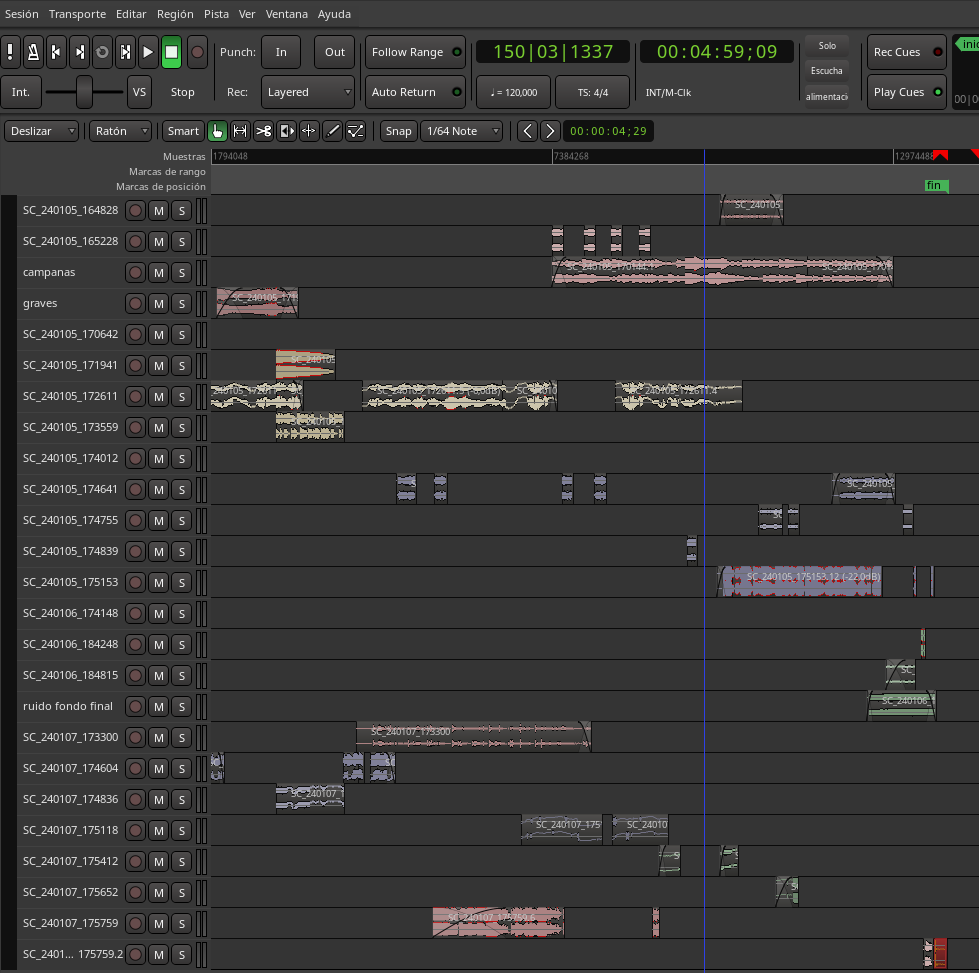
\includegraphics[width=0.8\textwidth]{./figuras/ardour.png}
%     \source{\propio}
%     \label{fig:ardour}
% \end{figure}


\section{Proceso y criterios de selección de material sonoro}

La selección de los fragmentos de código a utilizar en la composición se realizó en un momento posterior al de la propia generación, hasta dos meses más tarde en algunos casos, sin atender a las intenciones primeras a la hora de dialogar con la \gls{api} ni a su grado de adecuación a las peticiones. Se priorizó, más bien, la variedad de texturas y timbres, así como la posibilidad de combinarlos entre sí en un discurso sonoro coherente y equilibrado. La búsqueda se realizó escuchando bloque por bloque y renderizando a archivos de audio una o varias versiones de los mismos, ya que en ocasiones el resultado sonoro dependía de factores externos al código como la posición o el movimiento del ratón en los ejes $x$ e $y$ para modular ciertos parámetros del código. 

En el momento de la selección, se intentó diseñar una estructura base esquemática para la pieza con la ayuda de GPT-4, pero siempre surgían problemas asociados al entendimiento de los procesos en el tiempo por parte del \gls{llm}. Todas las soluciones propuestas por el \gls{llm} eran extremadamente simples en el mejor de los casos, y casi siempre lejos de lo que se pretendía, a saber, una composición temporal a partir de samples. Por esta razón, se optó por la intervención humana absoluta en el proceso de composición, relegando el papel de GPT-4 a la generación de material sonoro\footnote{El anexo \ref{anexo:algorai} contiene los materiales sonoros elegidos para esta composición.}.

\section{Descripción de la pieza}

\emph{AlgorAI}\footnote{La pieza puede ser escuchada en los enlaces del código QR de la Figura \ref{fig:sonograma_algorai}} es una obra de música electroacústica cuyos materiales provienen de código de programación. Su duración es de 5 minutos y está compuesta de un único movimiento, sin secciones claramente delimitadas. Su trama está compuesta por una sucesión polifónica de texturas sonoras de diversa índole, que se van superponiendo y combinando entre sí (véase una sección del sonograma de la Figura \ref{fig:sonograma_algorai}). Las decisiones de posición, duración y altura de cada sonido han sido tomadas en conjunto por el propio compositor, atendiendo a criterios de equilibrio, coherencia e inteligibilidad desde el punto de vista psicoacústico. Su título, \emph{AlgorAI}, es un acrónimo de \emph{Algoritmo} e \emph{Inteligencia Artificial}, y hace referencia a la naturaleza de la obra, cuya materia prima sonora ha sido compuesta a partir de algoritmos de IA, en concreto, por grandes modelos de lenguaje. Al mismo tiempo, hace un guiño al término \emph{Algorave}, asociado a la práctica del \emph{live coding}\footnote{Según Wikipedia, <<Una \emph{algorave} (de \emph{algoritmo} y \emph{rave}) es un evento en el que la gente baila con música generada a partir de algoritmos, a menudo utilizando técnicas de codificación en vivo>> \citep{Algorave2023}.}.  Los materiales sonoros son en su mayoría de origen íntegramente electrónico (aquellos producidos a través de SuperCollider), y en menor medida, de origen electroacústico (los producidos por Tidal Cycles), cuando la base de los mismos es un conjunto de sonidos muestreados.


\section{Técnicas de síntesis sonora utilizadas en los materiales sonoros}

Síntesis sustractiva\footnote{La síntesis sustractiva consiste en eliminar ciertas frecuencias de un sonido rico en armónicos, como el ruido blanco, mediante el uso de filtros, para crear sonidos con características tonales específicas \citep{AcademiaLabSustractiva}.}, síntesis aditiva\footnote{La síntesis aditiva crea sonidos complejos mediante la suma de ondas sinusoidales individuales, cada una con su propia frecuencia, amplitud y fase, imitando así la forma en que los sonidos naturales se componen de armónicos \citep{AcademiaLabAditiva}.}, frecuencia modulada\footnote{La síntesis de frecuencia modulada (FM) implica la modulación de la frecuencia de una onda portadora por otra onda, llamada moduladora, creando una amplia gama de armónicos y sonidos complejos \citep{AcademiaLabFM}.}, granulación\footnote{La síntesis granular trabaja con pequeños fragmentos de sonido, o "granos", que se manipulan y reorganizan para crear texturas sonoras complejas y evolutivas \citep{AcademiaLabGranular}.} y amplitud modulada\footnote{La síntesis de amplitud modulada (AM) implica modificar la amplitud de una señal sonora (portadora) con otra señal (moduladora), resultando en la aparición de nuevas frecuencias o armónicos \citep{AcademiaLabAM}.} son, en ese orden, las técnicas de síntesis sonora más utilizadas por GPT-4 a lo largo del trabajo, en lo que la utilización del lenguaje de SuperCollider se refiere, independientemente de la petición del usuario en los prompts. La Figura \ref{fig:grafica_sintesis_gpt4} muestra esta distribución de uso de las técnicas de síntesis sonora utilizadas en los fragmentos de código que han servido como base de la composición. Se aprecia una tendencia a la síntesis sustractiva, aquella que consiste en filtrar armónicos de un sonido complejo, generalmente ruido blanco o clics, para obtener sonidos complejos y ricos en matices.

\begin{figure}[H]
    \caption[Gráfica circular con la distribución de las técnicas de síntesis sonora utilizadas en los materiales sonoros generados por GPT-4 en SuperCollider]{Gráfica circular con la distribución de las técnicas de síntesis sonora utilizadas en los materiales sonoros generados por GPT-4 en SuperCollider.}
    \centering
    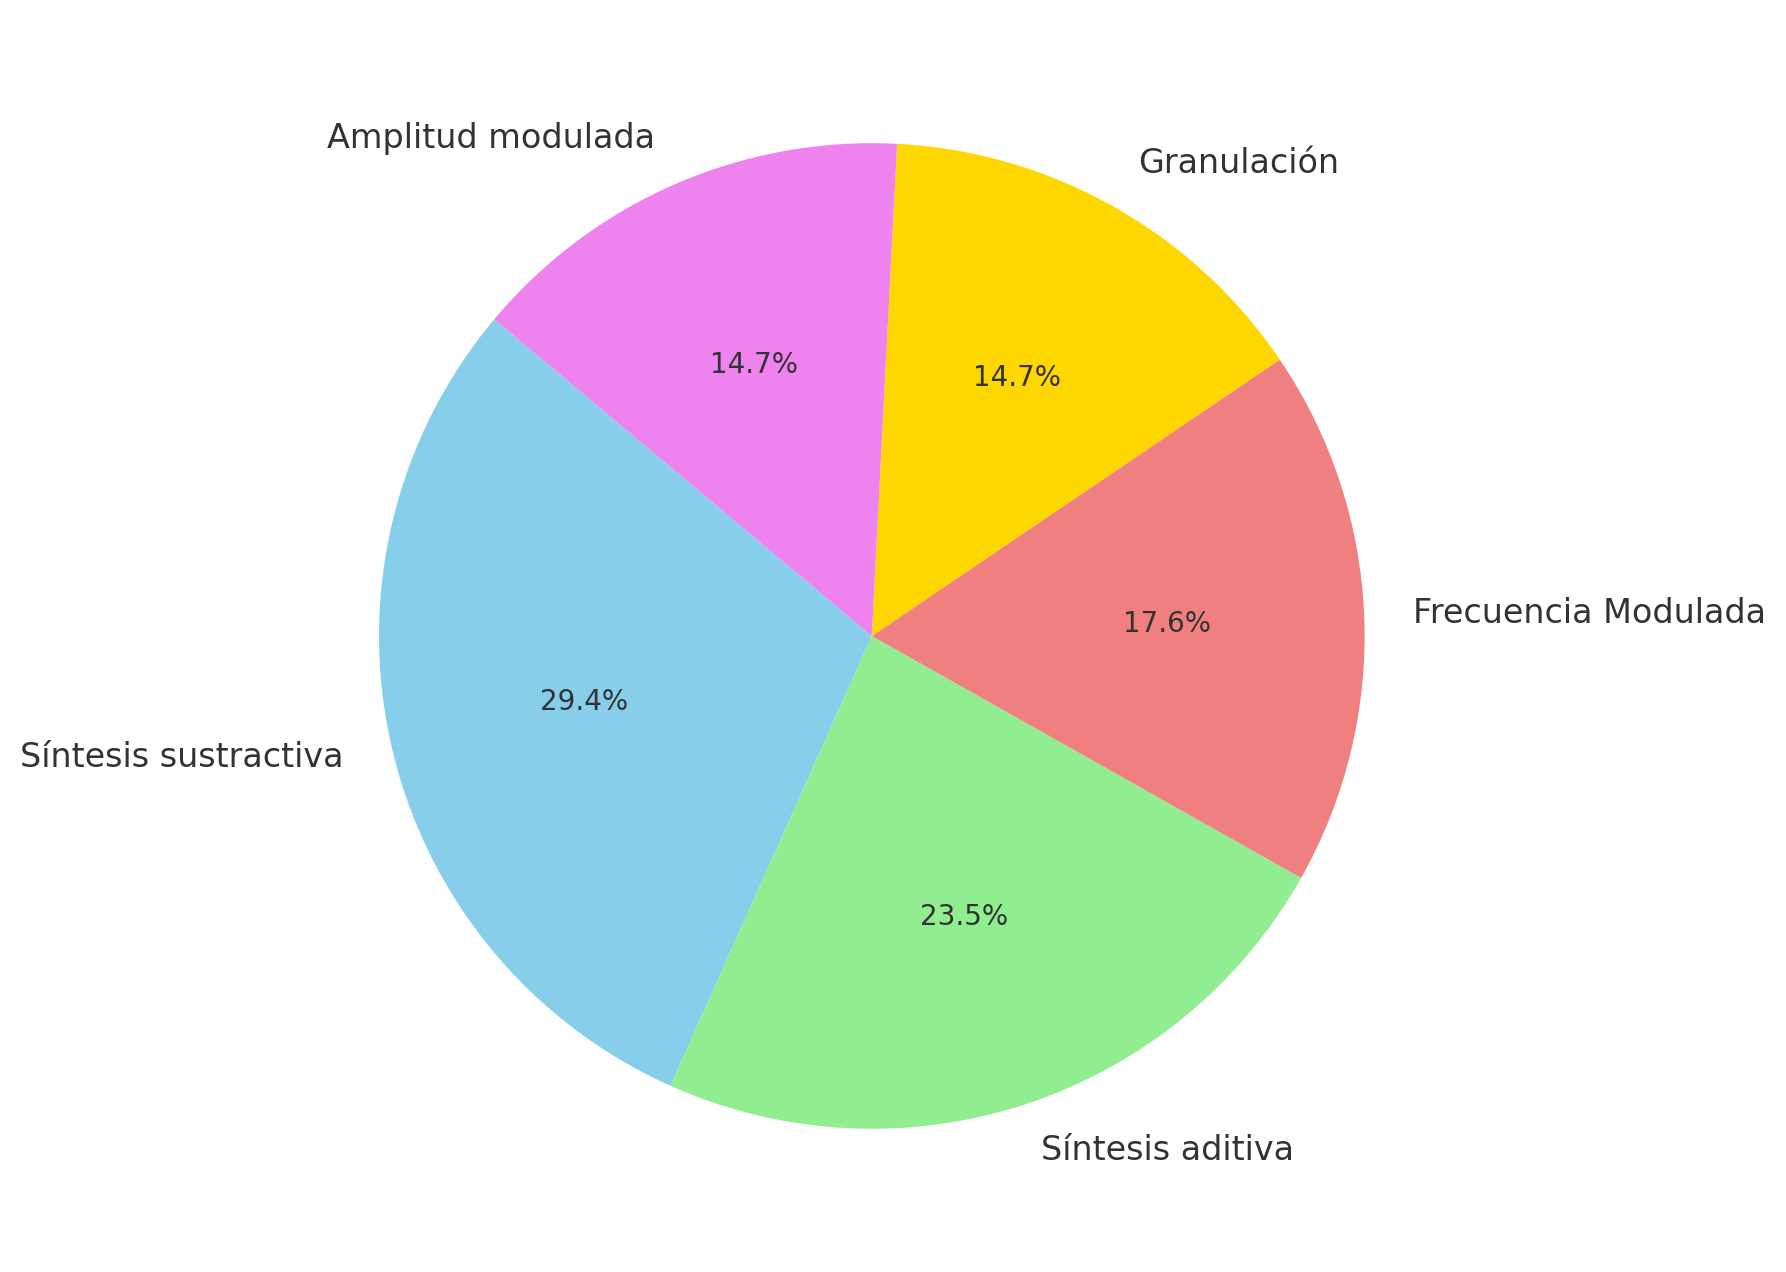
\includegraphics[width=0.7\textwidth]{./figuras/grafica_sintesis_gpt4_quesitos.png}
    \note{Se aprecia cierta tendencia a la utilización de la síntesis sustractiva.}
    \source{\propio}
    \label{fig:grafica_sintesis_gpt4}
\end{figure}

Una parte significativa de los materiales sonoros, a pesar de estar generados aparentemente por una técnica definida, en realidad deben su sonido más bien a combinaciones casuales y complejas, más fruto del azar que de la intención. Esto es común cuando los diversos parámetros de un sistema son llevados al extremo y producto sonoro es fruto de artefactos digitales como saturaciones, \emph{aliasing}, etc. Este aspecto de serendipia e impredecibilidad en la utilización de modelos de lenguaje aplicados a lo sonoro no es desdeñable, ya que puede ser una fuente de inspiración para el compositor.

Es notoria la naturaleza distinta en los materiales generados en el lenguaje de Tidal Cycles respecto a SuperCollider, ya que aquel se basa en la manipulación de samples y en su secuenciación en el tiempo en bucles. Los bucles más complejos que se aprecian en \emph{AlgorAI} han sido producidos por GPT-4 en Tidal Cycles. En este caso, a criterio personal del investigador, se han priorizado siempre los bucles sonoros más impredecibles, aquellos que no se ajustan a una estructura rítmica regular. La Figura \ref{fig:ejemplo_tidal_irregular} muestra uno de los ejemplos escritos en Tidal Cycles escogidos para la composición por su carácter irregular.



\begin{figure}[H]
    \captionqr{Ejemplo de código en Tidal Cycles escogido para la composición por su carácter irregular e impredecible}{Ejemplo de código en Tidal Cycles escogido para la composición por su carácter irregular e impredecible.}{https://drive.google.com/file/d/11KYkFOkBN42MlXUgHlmI8Rk2RWT7gQ8f/view?usp=drive_link}{audio}
    \centering
    \setstretch{1}
    \begin{lstlisting}[style=SuperCollider-IDE, language=ExtendedHaskell, basicstyle=\footnotesize\ttfamily, numbers=none]
d1 
    $ degradeBy 0.1
    $ slow 10 
    $ n (struct "[t(3,8)]*3 t(5,6) [t(6,7)]*4 t(3,4) t(2,3) t(7,8)"
        $ slow 3 
        $ ((fast 3 sine * rand) * (1-(fast 5 tri)) * (1-(fast 45 tri * rand))) *20) 
            # s "[[rash, cpu] | cpu2 | numbers | [arpy, <hi lo snare>] | [superpiano, [alphabet clap]?]]" 
            -- # s (choose["[rash, cpu]" , "[cpu2, hc]" ,"numbers" ," [arpy, <hi lo snare>]" , "[superpiano, [alphabet clap]?]"])
            # speed (slow 7 $ sine*1+0.05) 
            # legato 10
            # squiz (slow 20 $ sine*5)
            # room 1
            # size 0.8
            # delay 0.8
            # delaytime (choose [0.1, 0.5, 1])
            # delayfb 0.8
            # pan (range 0 1 rand)
            # vowel (slow 2.7 "{u o i e a i u a, a e i o u o}")
    \end{lstlisting}
    \source{\propio}
    \label{fig:ejemplo_tidal_irregular}
\end{figure}

\section{Interacción humano-LLM en el proceso de composición}

En este punto surge la cuestión de si la inteligencia artificial ha influenciado la orientación y el resultado final de la composición musical. Desde la perspectiva del autor de la misma, que simultáneamente desempeña un papel de investigador, se concluye que la respuesta es negativa. La metodología empleada para la mixtura temporal de los diversos elementos sonoros, incluyendo su segmentación, extensión, secuenciación, entre otros, es resultado de un proceso de decisión consciente y creativa por parte del compositor. Es preciso señalar que el uso de materiales alternativos habría conducido a la creación de una obra distinta, si bien manteniendo un carácter y estilo semejantes.

No obstante, no podemos subestimar el impacto que la incorporación de materiales sonoros originados por \gls{ia} representa en el proceso creativo. En primera instancia, esta inclusión ha facilitado al compositor-investigador el descubrimiento de texturas y matices tímbricos inéditos, los cuales no habrían sido factibles de hallar mediante métodos convencionales. Tradicionalmente, el artista sonoro se aventura en la búsqueda de sus materiales sonoros, ya sea capturando sonidos del entorno real mediante dispositivos de grabación o experimentando en el ámbito electrónico o digital con herramientas como sintetizadores, secuenciadores y software especializado en la generación de sonido. La exploración a través de \gls{lm} programáticos ha posibilitado la identificación de materiales inaccesibles para el compositor por sí solo, no por una limitación en sus competencias técnicas, sino debido a que la diversidad de combinaciones posibles de elementos generativos es inabarcable. Además, el ser humano tiende a replicar patrones y estructuras previamente exitosos o familiares, con lo que una herramienta de \gls{ia} puede beneficiar a la variedad en el proceso de generación de materiales sonoros originales.

Cabe destacar la reducción significativa en la carga de trabajo que ha representado el empleo de \gls{llm} para la generación de materiales sonoros, minimizando el tiempo requerido en comparación con métodos tradicionales de creación. Podría argumentarse que esto conlleva a una pérdida del control artístico sobre la obra; sin embargo, esta afirmación no es necesariamente acertada. La actitud del compositor hacia la interacción con el \gls{llm} a través de sus distintas interfaces se ha caracterizado por un proceso de selección y búsqueda constante. De los códigos generados, solo una fracción de los bloques sonoros ha sido seleccionada para la composición, tras un procedimiento de descarte basado en la audición y criterios estéticos subjetivos. Los fragmentos finalmente incorporados son el resultado de múltiples iteraciones de diálogo con el modelo. En el contexto de la música experimental, la incorporación de elementos externos a la intención original del compositor constituye una práctica habitual, y la utilización de \gls{llm} emerge como una herramienta a tener en cuenta en la exploración sonora.

